\documentclass[11pt,a4paper]{article}
\usepackage{ls}
\usepackage[utf8]{inputenc}

\title{Business Process Landscaping}

\author{Toni Pfeiffer\\[.3cm] Universität Leipzig -- Seminar Complex Systems
  and Co-operative Action }

\date{November 28, 2021}

\begin{document}

\maketitle

\section{Business Process Landscape}

A large part of process management deals with the identification and selection
of processes that run in a company. According to ISO 9001, a company is
obliged to document all processes and to present them in a suitable form. A
tool to draw these processes and to navigate through the process landscape of
a company is the process map.

A process map is a graphical overview of all business processes in a company
and is intended to present the processes in a structured, simple, clear and
understandable way. A distinction can be made between process maps for the
entire organization and for individual departments of the company.
Accordingly, process maps can exist in different resolutions and forms of
presentation. The process map shows the flow of the processes and is
independent of the structure of the company. Thus, there can also be
illustrations that go beyond departmental boundaries or also include the
customer. An organization chart shows who does what. A process map, on the
other hand, shows how something is done. The process map is a guide to process
optimization and shows the interfaces and interactions between processes.

Important parameters for the creation of process maps are the following:

\begin{itemize}
\item Input and Output
\item Sequence and Interaction
\item KPI's
\item Resources and Responsibilities
\item Risks and Opportunities
\item Competencies and Authorities
\item Documents and Methods
\item Changes
\item Methods of Monitoring, Measurement and Evaluation
\item Opportunities of Improvement
\end{itemize}

A process map is important for many stakeholders. These include employees,
management, certifiers, consultants, customers and all other parties. In
fig.~\ref{BPL} you can see schematically all important components. The
processes are roughly divided into 3 different types, the management
processes, the core processes and the support processes. What makes up these
types and how they can be distinguished is discussed in more detail in section
\ref{sec:process}.

\begin{figure}[h] 
  \centering
     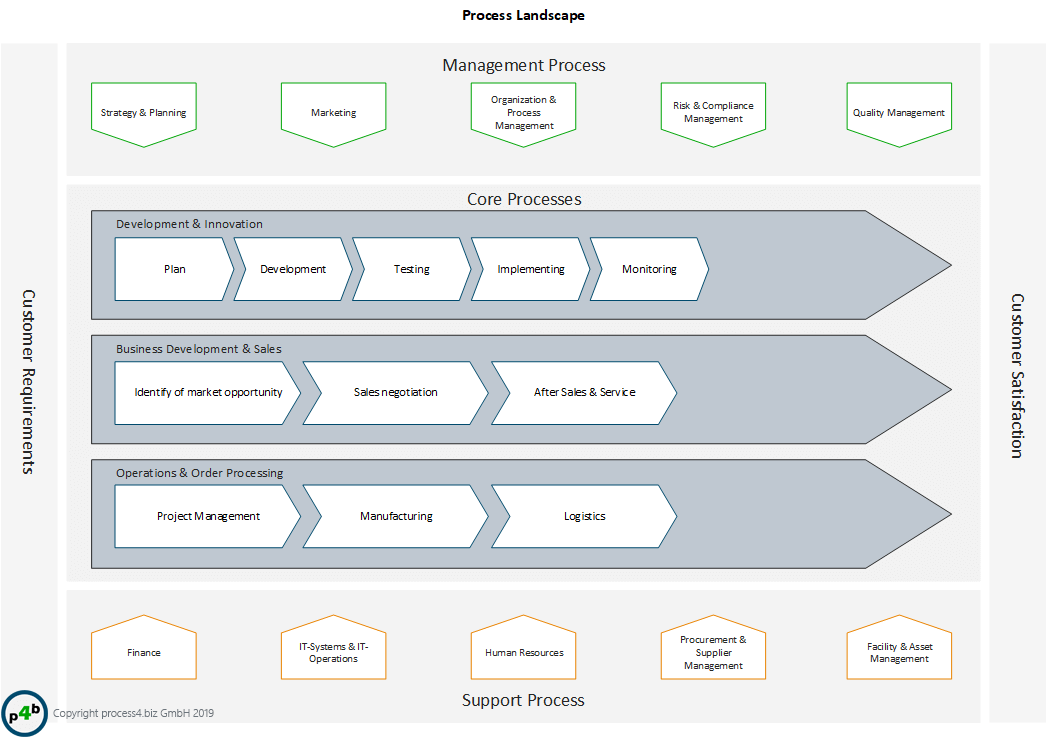
\includegraphics[width=\textwidth]{plk.en.png}
  \caption{Business Process Landscape \cite{7}}
  \label{BPL} 
\end{figure}

\subsection{Static and Dynamic}

In fig.~\ref{BPL} you can see a static business process map. Static process
maps tend to be the norm, but dynamic maps are on the rise in recent years. A
static map is a fixed diagram. All processes are mapped. The static process
map is initially modeled and further developed. A distinction is made between
end-to-end process maps and customer journey approaches. In the case of the
end-to-end process as shown schematically in fig.~\ref{BPL}, the output of one
process serves as the input of another process. These are shown from customer
requirements to customer satisfaction.

The customer journey approach aims to show all process steps that directly
affect the customer. In fig.~\ref{customer}, a customer journey map for online
shopping is shown. The customer focus can be clearly seen here.

\begin{figure}[h] 
  \centering
     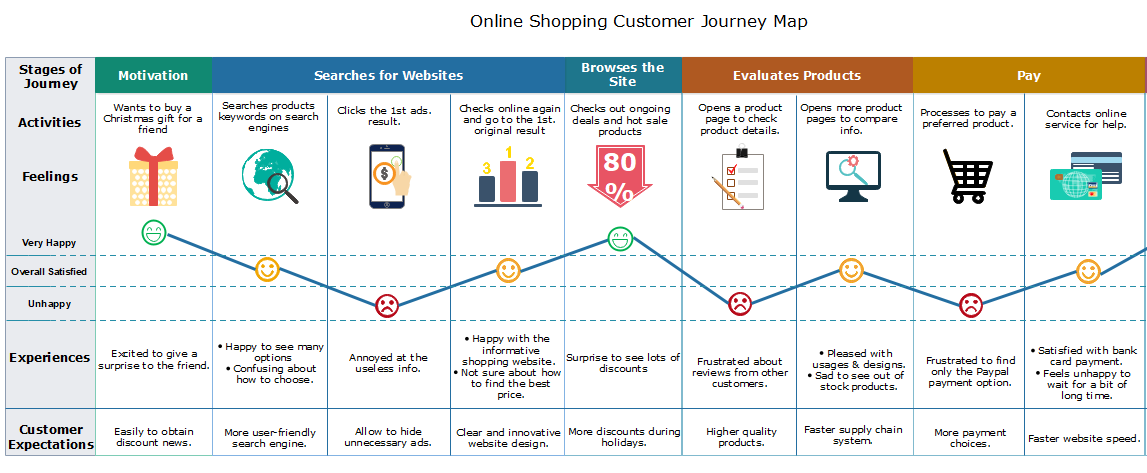
\includegraphics[width=\textwidth]{customer-journey-map.png}
  \caption{Customer Journey Map \cite{8}}
  \label{customer}
\end{figure}

Unlike static process maps, dynamic maps can change their view. In this case,
the map is generated automatically based on predefined properties. For
example, an employee may only see the processes of his or her location.
Dynamic maps are freely configurable and offer many advantages, especially for
companies with global operations. It is possible to display distributed
processes and visualize their interaction. A popular tool is the SMARTMAP,
where individual processes and process steps can be viewed by zooming in and
out.

\section{Process and kinds of processes}\label{sec:process}

In order to create a process map, one must first be able to recognize and
describe processes. This is done by dividing processes into 3
types. Management processes, core processes and support processes. According
to ISO 9001, the interaction of processes is also very important. This should
be recognized and included in the process optimization. For process
optimization, it also helps to identify the interfaces between processes.
These can be easily identified using the process map. In the following, the
different process types are presented and two methods for process description
are also examined in more detail.

\subsection{Management Process}

All strategic processes that take place in a company can be described as
management processes. Since these are not always tangible, it is difficult to
identify and describe them. There are usually a few processes that relate to
the entire company. They are particularly concerned with reporting,
organizing, planning, coordinating, instructing and controlling. Examples
would be internal audits, resource planning, the strategy process, defining
responsibilities, evaluating objectives, and managing the business.

Since it can prove difficult to identify these processes, already established
process management tools can also be used to develop a process map. One
example in relation to management processes is the Balanced Scoreboard. In
fig.~\ref{balance} such a scorecard is recorded.

You can see the 4 perspectives that characterize such a scoreboard. These are
the financial perspective, the customer perspective, the internal process
perspective and the learning and development perspective. A scoreboard
highlights the success factors and facilitates strategic decisions. Not only
financial but also monetary metrics are considered. This is to draw a
balanced, holistic and realistic picture of a company. The advantages are
transparency, a holistic view, clear communication and flexibility.

\begin{figure}[h] 
  \centering
     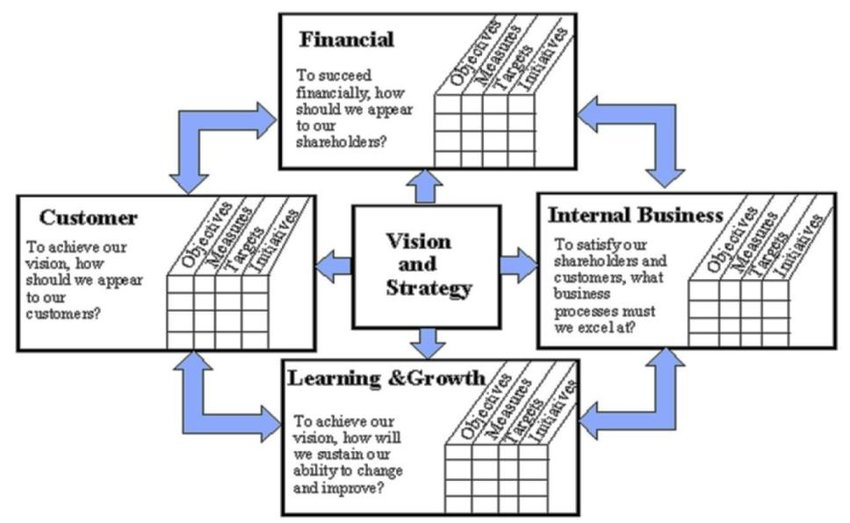
\includegraphics[width=\textwidth]{balanced-scorecard.png}
  \caption{Balanced Scoreboard \cite{9}}
  \label{balance}
\end{figure}

\subsection{Core Process}

Value creation processes are processes that directly create value and earn
money. They are the raison d'être of the company. Since they form the core of
the company, they are also called core processes. A core process in a process
map shows a sequence from creation to completion of a product or service. This
is mapped in a logical sequence and shows the uniqueness of the company. The
goal of the core processes is to satisfy the customer's needs. Examples of
core processes are service provision, design, production, development and
delivery of products.

\subsection{Support Process}

Support processes ensure that core processes are kept running. This includes
the provision of personnel, infrastructure and material. In the process, costs
are incurred that the customer pays for indirectly. Examples would be the
tracing of products, the maintenance of machines and systems, the
documentation and the processing of complaints.

\begin{thebibliography}{99}

% For books
\bibitem{1} \url{https://smct-management.de/prozesslandkarte/}

\bibitem{2}
  \url{https://prozessoptimierung-sprung.de/prozesslandkarte-erstellen/}

\bibitem{3}
  \url{https://www.business-wissen.de/hb/prozesslandkarten-erstellen/}

\bibitem{4}
  \url{https://www.weka.de/qualitaetsmanagement/prozesslandschaft-damit-haben-sie-den-ueberblick/}

\bibitem{5}
  \url{https://www.intellior.ag/drei-beliebtesten-prozesslandkarten-aus-der-praxis/}

\bibitem{6}
  \url{https://www.tuvsud.com/de-de/-/media/de/management-service/pdf/iso-9001/broschuere-iso-9001.pdf}

\bibitem{7}
  \url{https://process4.biz/en/corporate-documentation/process-landscape/plk.en.png}, [Online Stand 28.11.2021].

\bibitem{8}
  \url{https://images.edrawsoft.com/images2019/articles/customer-journey-examples/online-shopping-customer-journey-map.png}, [Online Stand 28.11.2021].

\bibitem{9}
  \url{https://www.researchgate.net/profile/Amna-Ascic/publication/318381043/figure/fig5/AS:668323012423687@1536352031365/BALANCED-SCORECARD-FRAMEWORK.jpg}, [Online Stand 28.11.2021].

\end{thebibliography}

\end{document}
